\chapter{Introduction to the RGB-D Visual Odometry Problem}%
\label{cha:rgbd_vo}

\minitoc%
\clearpage

\section{Modeling Image Capture in a Camera}%
\label{sec:image-formation}

\subsection{Historic Remarks}%
\label{sub:historic_remarks}

The study of the image formation process has a long history.
Traces of geometric formulations of image formation are present
in Euclid work (4th century B.C.) and partially correct perspective
projections are visible in frescoes of Pompeii (1 B.C.).
These skills also re-emerged in Renaissance art with artists such as
Brunelleschi, Donatello and Alberti.
A treatise on the projection process, \textit{``Della Pittura''},
was published by Leon Battista Alberti in 1435 and influenced
many Renaissance artists such as Leonardo da Vinci and Raphael.
In Figure~\ref{fig:raphael_school_athens}
the perspective emerges from the vanishing point.
D\"urer devised a machine to get a perspectively correct image,
represented in Figure~\ref{fig:durer_perspective_machine}.
It is a manual reproduction of what a camera does today.

\begin{figure}[h]
\centering
\begin{subfigure}[b]{0.48\textwidth}
	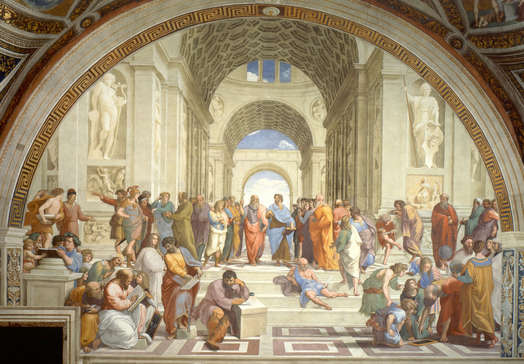
\includegraphics[width=\textwidth]{assets/img/raphael_school_athens.jpg}
	\caption{Raphael, The School of Athens (1509)}%
	\label{fig:raphael_school_athens}
\end{subfigure}
\hfill
\begin{subfigure}[b]{0.46\textwidth}
	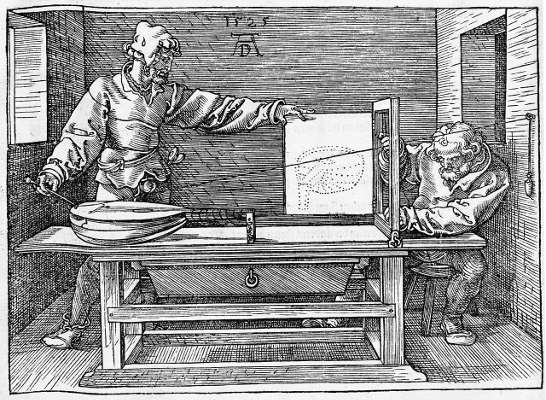
\includegraphics[width=\textwidth]{assets/img/durer_perspective_machine.jpg}
	\caption{D\"urer's perspective machine (1525)}%
	\label{fig:durer_perspective_machine}
\end{subfigure}
\caption{Usage of perspective projection in Renaissance art.}%
\end{figure}

Many artists also played with those perspective rules to create images
that seem locally correct but have inconsitent global depth or gravity
such as Hogarth (Figure~\ref{fig:hogarth_satire})
and Escher (Figure~\ref{fig:escher_belvedere}).

\begin{figure}[h]
\centering
\begin{subfigure}[b]{0.52\textwidth}
	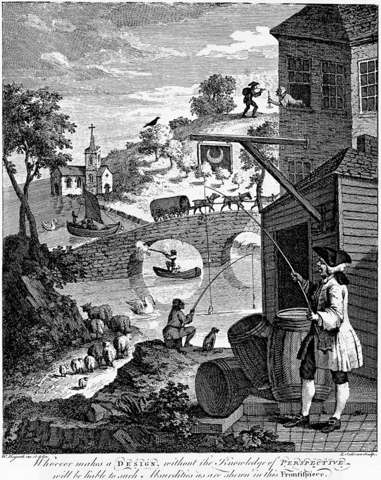
\includegraphics[width=\textwidth]{assets/img/hogarth_satire.jpg}
	\caption{Satire by Hogarth 1753}%
	\label{fig:hogarth_satire}
\end{subfigure}
\hfill
\begin{subfigure}[b]{0.42\textwidth}
	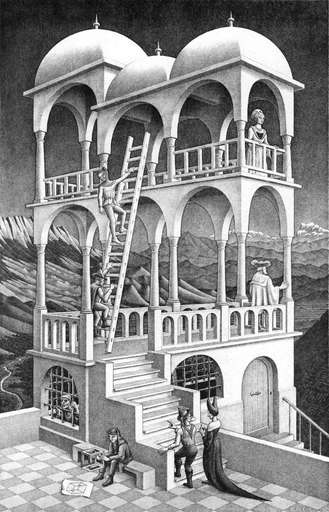
\includegraphics[width=\textwidth]{assets/img/escher_belvedere.jpg}
	\caption{Escher, Belvedere 1958}%
	\label{fig:escher_belvedere}
\end{subfigure}
\caption{Conscious circumvention of perspective projection in art.}%
\end{figure}


\subsection{Projective Geometry}%
\label{sub:projective_geometry}


In order to formally write transformations by linear operations,
we make extensive use of homogeneous coordinates to represent
3D point as a 4D-vector $(X,Y,Z,1)$ with the last coordinate fixed to 1.
This normalization is not always necessary. One can represent 3D points
by a general 4D vector
\[
	\bm{X} = (XW, YW, ZW, W)\ \in\ \R^4.
\]
In general, an n-dimensional projective space $\mathbb{P}^n$
is the set of all one-dimensional subspaces (i.e.\ lines through the origin)
of the vector space $\R^{n+1}$.
A point $p \in \mathbb{P}^n$ can then be assigned homogeneous coordinates
$\bm{X} = \tr{(x_1, \ldots, x_{n+1})}$, among which at least one $x$ is nonzero.
For any nonzero $\lambda \in \R$, the coordinates
$\bm{Y} = \tr{(\lambda x_1, \ldots, \lambda x_{n+1})}$
represent the same point $p$.


\subsection{Pinhole Camera Model}%
\label{sub:pinhole}


\begin{figure}[h]
\centering
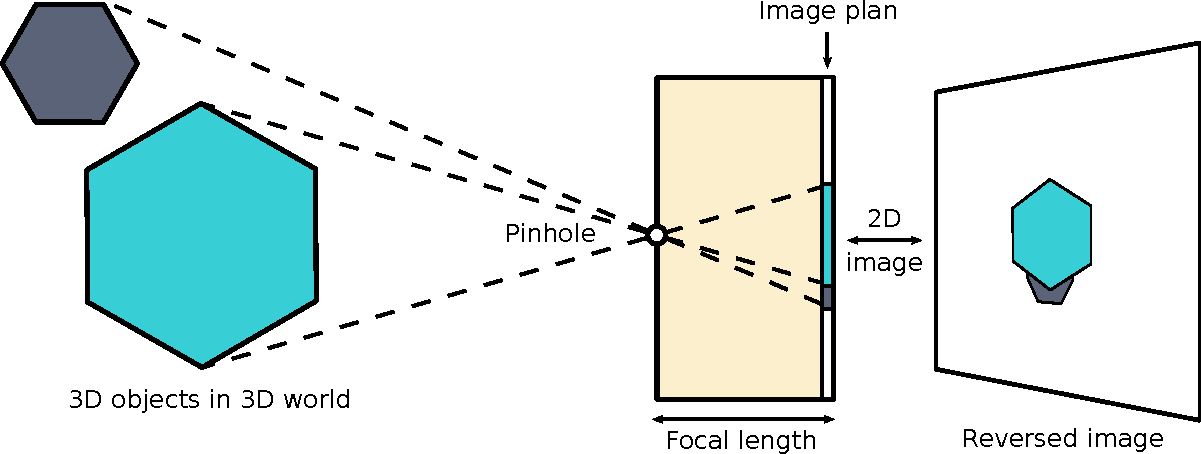
\includegraphics[width=\textwidth]{assets/img/pinhole.pdf}
\caption{Pinhole camera model.}%
\label{fig:pinhole_camera}
\end{figure}

Perspective projection emerges from a simplified model
of a real camera called the pinhole camera,
represented in Figure~\ref{fig:pinhole_camera}.
The main issue of such a camera,
is that the hole has to be very small to get a sharp image,
preventing light to enter the capture device.
In order to augment the amount of light, today we use lenses,
but just as with a pinhole camera, the image is upside down in the image plan.
In order to avoid dealing with minus signs in the equations,
we pretend that the image plan is virtually on the same side than the object.
The perspective transformation $\pi$ modeling this projection is given by
\[ \pi : \R^3 \rightarrow \R^2; \quad
	\bm{X} \mapsto x = \pi(\bm{X}) =
	\begin{pmatrix}
		f \frac{X}{Z} \\
		f \frac{Y}{Z} \\
	\end{pmatrix}
\]
where $f$ is the focal length, $X,Y,Z$ are the object coordinates
in the 3D world, the $z$ axis being the camera axis.
The one challenge we have to overcome, is that this transformation is non linear.
In order to do so, we use homogeneous coordinates,
which is basically similar to multiplying everything by $Z$,
\[ Z \bm{x} = Z \begin{pmatrix} x \\ y \\ 1 \end{pmatrix} =
	\begin{pmatrix}
		f & 0 & 0 & 0 \\
		0 & f & 0 & 0 \\
		0 & 0 & 1 & 0 \\
	\end{pmatrix}
	\begin{pmatrix}
		X \\ Y \\ Z \\ 1
	\end{pmatrix}
	= K_f \Pi_0 \bm{X}
\]
where we have introduced the two matrices
\[K_f =
	\begin{pmatrix}
		f & 0 & 0 \\
		0 & f & 0 \\
		0 & 0 & 1 \\
	\end{pmatrix}
	\quad \text{and} \quad
	\Pi_0 =
	\begin{pmatrix}
		1 & 0 & 0 & 0 \\
		0 & 1 & 0 & 0 \\
		0 & 0 & 1 & 0 \\
	\end{pmatrix}.
\]
The matrix $\Pi_0$ is referred to as the standard projection matrix.
We often note the distance to the camera along its axis with $\lambda > 0$ so
\[
	\lambda \bm{x} = K_f \Pi_0 \bm{X}.
\]


\subsection{Intrinsic Parameters}%
\label{sub:intrinsic_parameters}


If the camera is not centered at the optical center, we have an additional
translation $o_x, o_y$. The point where the optical axis intersects
the image plan is called the principal point.
If pixels do not have unit scale, we need to introduce
additional scaling factors $s_x$ and $s_y$.
And if pixels are not rectangular, we also have a skew factor $s_{\theta}$.
The transformation from coordinates in the frame of the camera
to final pixel coordinates has thus the following steps
\[
	\text{Camera}\ (\text{3D}, \bm{X})
		\quad \overset{K_f\Pi_0}{\longrightarrow} \quad
			\text{Image}\ (\text{2D}, \bm{x})
		\quad \overset{K_s}{\longrightarrow} \quad
			\text{Pixel}\ (\text{2D}, \bm{x'}).
\]
where the pixel coordinates $\bm{x'} = (x',y',1)$ are given by
$\lambda\ \bm{x'} = K_s\ K_f\ \Pi_0\ \bm{X}$
with
\[K_s = \begin{pmatrix}
		s_x & s_{\theta} & o_x \\
		0 & s_y & o_y \\
		0 & 0 & 1 \\
	\end{pmatrix}
	\quad \text{and} \quad K_f =
	\begin{pmatrix}
		f & 0 & 0 \\
		0 & f & 0 \\
		0 & 0 & 1 \\
	\end{pmatrix}.
\]
We call $K = K_s\ K_f$ the intrinsic matrix since it holds
parameters intrinsic to the camera system, independent from
the outside 3D world.


\subsection{Radial Distortion}%
\label{sub:radial_distortion}

The intrinsic parameters in the matrix $K$ model linear distortions
in the transformation to pixel coordinates.
In practice however, one can also encounter significant
distortions along the radial axis.
This is particularly visible in a wide field of view
or if one uses cheaper cameras such as webcams.
A simple effective model for such distortions is to use
\[
	x = x_d ( 1 + a_1 r^2 + a_2 r^4 ),\quad
	y = y_d ( 1 + a_1 r^2 + a_2 r^4 )
\]
where $\bm{x} = (x_d, y_d)$ is the distorted point,
and $r^2 = \|\bm{x}\|^2$ is its squared distance to the principal point.
Usually, $a_1$ and $a_2$ are estimated through a calibration step computed from
distortions of straight lines as in Figure~\ref{fig:radial_distortion}
or simultaneously with a 3D reconstruction~\cite{stein1997lens, fitzgibbon2001simultaneous}.
Other more sophisticated models exist~\cite{devernay1995automatic}
but we will not enter in details here since we will consider
that images are rectified as if fitting the pinhole model.

\begin{figure}[h]
\centering
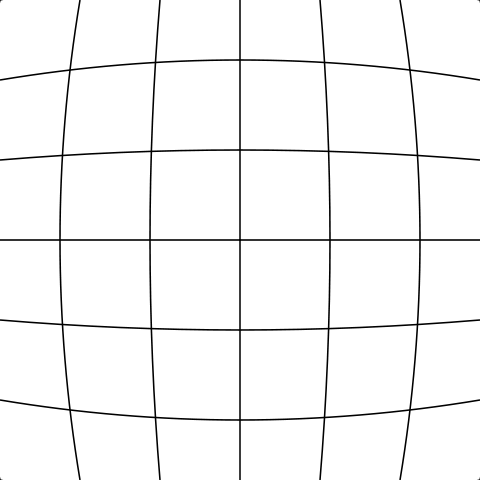
\includegraphics[width=0.5\columnwidth]{assets/img/barrel_distortion.png}
\caption{Grid projection with radial distortion.}%
\label{fig:radial_distortion}
\end{figure}


\section{Modeling Camera Movements}%
\label{sec:moving-scene}

\subsection{Origins of Visual Odometry}%
\label{sub:origins_of_visual_odometry}

Aiming to reconstruct a three-dimensional structure of the world from
a set of two-dimensional views has a long history in computer vision.
It is generally considered and ill-posed problem since reconstructions
consistent with a given set of observations/images are typically not unique.
Therefore, one need to impose additional assumptions.
The study of geometric relations between a 3D scene
and observed 2D projections is based on two types of mathematic transformations, namely
\begin{itemize}
	\item Perspective projection, and projective geometry to account for the image formation
		process we presented in the previous section.
	\item Euclidean motion or ``rigid body motion''
		representing the motion of the camera from one frame to the next.
\end{itemize}

The first known work on the problem of multiple view geometry was that of
Erwin Kruppa (1913) who showed that two views of five points
are sufficient to determine both the relative tansformation
(``motion'') between the two views and the 3D location (``structure'')
of the points up to a finite number of solutions.
A linear algorithm to recover structure and motion from two views based
on the epipolar constraint was proposed by Longuet-Higgins in 1981~\cite{longuet1981computer}.
Several summarizing text books and papers were also written
on the subject~\cite{faugeras1993three, weng1993optimal}.
Extensions to three views~\cite{spetsakis1987closed, shashua1994trilinearity}
and factorization techniques for multiple views and orthogonal projection were
also developed~\cite{tomasi1992shape}.
Depending on communities and context,
the joint estimation of camera motion and surrounding 3D environment is called
structure and motion or visual SLAM (simultaneous location and mapping).
Visual SLAM techniques slightly differ from structure and motion in the sense
that they are specialized for timely coherent sequences of images such as videos.
Visual odometry, that we will detail later, is the core step of Visual SLAM,
consisting of evaluating the camera motion of the next frame in the sequence.
Structure and motion however usually refers to situations where no such assumption
is done regarding the set of images.

\subsection{3D Space \& Rigid Body Motion}%
\label{sub:3d_space_rigid_body_motion}

\subsubsection{Three-dimensional Euclidean Space}%
\label{ssub:three_dimensional_euclidean_space}

The three-dimensional Euclidean space $\E^3$ consists of all points
$p \in \E^3$ characterized by coordinates
$\bm{X} = \tr{(X_1, X_2, X_3)} \in \R^3$
such that $\E^3$ can be identified with $\R^3$.
By identifying $\E^3$ and $\R^3$,
one can endow $\E^3$ with a scalar product, a norm and a metric.
This allows to compute distances, curve lengths, areas and volumes.


\subsubsection{Cross Product \& Skew-symmetric Matrices}%
\label{ssub:cross_product_and_skew_symmetric_matrices}

The cross product of two vectors $\bm{u}$ and $\bm{v}$ in $\R^3$ is a vector orthogonal to both.
\[
	\times : \R^3 \times \R^3 \rightarrow \R^3,\quad \bm{u} \times \bm{v} =
	\begin{pmatrix}
		u_2v_3 - u_3v_2 \\
		u_3v_1 - u_1v_3 \\
		u_1v_2 - u_2v_1
	\end{pmatrix} \in \R^3.
\]
Since $\bm{u} \times \bm{v} = -\bm{v} \times \bm{u}$, the cross product
also introduces an orientation.
Fixing $\bm{u}$ induces a linear mapping $\bm{v} \mapsto \bm{u} \times \bm{v}$
wich can be represented by the skew-symmetric matrix
\[
	\twist{u} = \cross{u} = \hatmat{u_1}{u_2}{u_3} \in \RR{3}{3}.
\]
such that $\bm{u} \times \bm{v} = \twist{u} \ \bm{v}$.
In turn, every skew symmetric matrix $M \in \RR{3}{3}$
verifying $M = -\tr{M}$
can be identified by a vector $\bm{u} \in \R^3$.
The operator $\wedge$ (``hat'') defines an isomorphism between $\R^3$
and the space $\sooo$ of the $3 \times 3$ skew-symmetric matrices.
Since a similar property is true for twists that we introduce later,
we will use the notation $\cross{u}$ instead of $\twist{u}$,
which is a visual reminder that it acts like a cross product.
Its inverse is denoted by (``vee'') $\vee : \sooo \rightarrow \R^3$.


\subsubsection{Rigid-Body Motion}%
\label{ssub:rigid_body_motion}

A rigid-body motion (or rigid-body transformation)
is a family of maps preserving the norm and cross product of any two vectors.
\begin{gather*}
	g : \R^3 \rightarrow \R^3,\quad \bm{u} \mapsto g(\bm{u}), \\
	\forall \bm{u} \in \R^3, \quad \|g(\bm{u})\| = \|\bm{u}\|, \\
	\forall\ \bm{u},\bm{v} \in \R^3, \quad g(\bm{u}) \times g(\bm{v}) =
		g(\bm{u} \times \bm{v})
\end{gather*}
Since norm and scalar product are related by the polarization identity
one can also state that a rigid-body motion is a map which
preserves inner product and cross product.
As a consequence, rigid-body motions also preserve the triple product,
and therefore volumes.
\[
	\forall\ \bm{u}, \bm{v}, \bm{w} \in \R^3, \quad
	\inner{g(\bm{u})}{g(\bm{v}) \times g(\bm{w})} =
		\inner{\bm{u}}{\bm{v} \times \bm{w}}.
\]

Let $\bm{e_1}, \bm{e_2}, \bm{e_3} \in \R^3$
be the orthonormal oriented vectors of our initial frame.
We note the transformed vectors $\bm{r_i} = g(\bm{e_i})$
and $R$ the matrix $R = (\bm{r_1}, \bm{r_2}, \bm{r_3})$
The first constraint (preservation of scalar product) implies that
$R$ is an orthogonal matrix $\tr{R}R=R\tr{R}=I$.
The second property (preservation of cross product) implies that $\det(R) = +1$.
In other words, $R$ is an element of the group
$SO(3) = \Set{R \in \RR{3}{3}} {\tr{R}R=I,\ \det(R) = +1}$.
The motion of the origin can be represented by a translation $\bm{t} \in R^3$.
Thus the rigid-body motion $g$ can be written as
\[
	g(\bm{x}) = R\bm{x} + \bm{t},\quad R \in SO(3),\quad \bm{t} \in \R^3.
\]

\subsubsection{Image Formation with Camera Movement}%
\label{ssub:projectionWithMovement}

Let's consider $\bm{X_0}$ a point in the World reference frame.
Its coordinates in the camera frame are determined by a rigid body motion
$\bm{X} = g(\bm{X_0}) = R \bm{X_0} + \bm{t}$.
In homogeneous coordinates, we can write
$\bm{X} = g\bm{X_0} = \inmatrix{ R & \bm{t}\\ 0 & 1} \bm{X_0}$.
In~\ref{sub:intrinsic_parameters}, we identified that pixels coordinates
are linked to point coordinates in the camera frame by
$\lambda\ \bm{x'} = K_s\ K_f\ \Pi_0\ \bm{X}$.
In total, the transformation from World coordinates to pixels coordinates
is given in homogeneous coordinates by
\[\boxed{
	\lambda\ \bm{x'} = K\ \Pi_0\ g\ \bm{X_0}
}\]
where $\lambda$ is the depth of the point in the camera frame,
$K$ is the intrinsics matrix, $\Pi_0$ the standard projection matrix
and $g$ the rigid body motion characterizing the camera,
also sometimes called extrinsics matrix.


\subsection{The Lie Group $SO(3)$ and Lie Algebra $\sooo$}%
\label{sub:the_lie_group_so_3}


\subsubsection{Sophus Lie (1841--1899)}%
\label{ssub:sophus_lie_1841_1899}

\begin{figure}[ht]
\centering
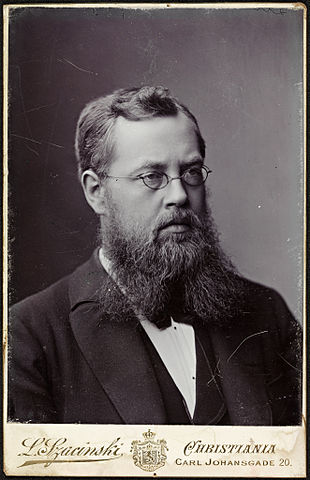
\includegraphics[width=10em]{assets/img/sophus_lie.jpg}
\caption*{Portrait of Marius Sophus Lie}
\end{figure}

Marius Sophus Lie was a Norwegian-born mathematician.
He created the theory of continuous symmetry, and applied it to
the study of geometry and differential equations.
He discovered that continuous transformation
groups are better understood in their linearized versions
(Theory of transformation groups, 1893).
These infinitesimal generators form a structure which is today
known as a Lie algebra.


\subsubsection{Lie Algebra $\sooo$}%
\label{ssub:lie_algebra_so3}

One can show that the effect of any infinitesimal
rotation $R \in SO(3)$ can be approximated by an element from
the space of skew-symmetric matrices
$\sooo = \Set{\cross{w}}{\bm{w} \in \R^3}$.
The rotation group $SO(3)$ is called a Lie group.
The space $\sooo$ is called its Lie algebra.


\subsubsection{The Exponential Map}%
\label{ssub:the_exponential_map}

Given the infinitesimal formulation of a rotation,
obtained from a continuous set of rotations $R(t)$
and by deriving the equation $R(t)\tr{R(t)} = I$,
one can show that $\dot{R}\tr{R}$ is a skew-symmetric matrix
and that we have the differential equation system
\[\left\{
	\begin{aligned}
		\dot{R}(t) &= \cross{w}(t)R(t), \\
		R(0) &= I. \\
	\end{aligned}
\right.\]
If we assume that $\cross{w}(t)$ is constant in time ($=\cross{w}$),
this known equation has the solution
\[
	R(t) = e^{\cross{w}t}
		= \sum_{n=0}^{\infty} \frac{{(\cross{w}t)}^n }{n!}
		= I + \cross{w}t + \frac{{(\cross{w}t)}^2 }{2!} + \ldots
\]
which is a rotation around the axis $\bm{w} \in \R^3$
by an angle of t (if $\|\bm{w}\| = 1$).
One can also absorb the scalar $t \in \R$ into the skew-symmetric matrix $\cross{w}$.
This matrix exponential therefore defines a map from
the Lie algebra to the Lie group
\[
	\exp : \sooo \rightarrow SO(3), \quad \cross{w}\mapsto e^{\cross{w}}.
\]
In analogy to the well-known Euler equation
$e^{i\theta} = \cos(\theta) + i \sin(\theta)$,
there is an expression called Rodrigues' formula for
the exponential of skew symmetric matrices,
\[
	e^{\cross{w}} = I + \frac{\cross{w}}{\|\bm{w}\|} \sin(\|\bm{w}\|)
		+ \frac{\cross{w}^2}{\|\bm{w}\|^2} (1 - \cos(\|\bm{w}\|)).
\]

\subsubsection{The Logarithm of $SO(3)$}%
\label{ssub:the_logarithm_of_so_3_}

There is conversely a mapping from the Lie group $SO(3)$ to the Lie algebra $\sooo$.
For any rotation matrix $R \in SO(3)$, there exists a vector $\bm{w} \in \R^3$
such that $R = \exp(\cross{w})$. Such an element is denoted by
$\cross{w} = \log(R)$. If $R \ne I$, we note $r_{ij}$ its coefficients
and $\bm{w}$ is given by
\[\left\{ \begin{aligned}
	\|\bm{w}\| &= \inv{\cos}\left(\frac{\text{trace}(R)-1}{2}\right),\\
	\frac{\bm{w}}{\|\bm{w}\|} &= \frac{1}{2\sin(\|\bm{w}\|)}
		\begin{pmatrix}
			r_{32} - r_{23} \\
			r_{13} - r_{31} \\
			r_{21} - r_{12} \\
		\end{pmatrix}.
\end{aligned}\right.\]
The above solution is not unique since for example,
increasing the angle by multiples of $2\pi$ will give the same rotation.


\subsection{The Lie Group $SE(3)$ and Lie Algebra $\seee$}%
\label{sub:the_lie_group_se_3}


\subsubsection{The Lie Algebra of Twists $\seee$}%
\label{ssub:the_lie_algebra_of_twists}

Just as with $SO(3)$ one can show that $SE(3)$
has a tangent space, of which the elements are called twists.
This tangent space is called the Lie algebra of twists, noted $\seee$.
\[
	\seee = \Set%
	{\twist{\xi} = \begin{pmatrix}\cross{w} & \bm{v} \\0 & 0 \end{pmatrix} \in \RR{4}{4}}
	{\cross{w} \in \sooo,\ \bm{v} \in \R^3}
\]

As with skew-symmetric matrices,
we can define operators ``hat'' $\wedge$ and ``vee'' $\vee$ to convert between
a twist $\twist{\xi} \in \seee$ and its coordinates $\bm{\xi} \in \R^6$.
The twist coordinates $\bm{\xi} = \inmatrix{\bm{v} \\ \bm{w}}$
are formed by stacking
the ``linear velocity'' $\bm{v} \in \R^3$ (related to translation)
and the ``angular velocity'' $\bm{w} \in \R^3$ (related to rotation).


\subsubsection{Logarithm and Exponential Coordinates for $SE(3)$}%
\label{ssub:exponential_coordinates_for_se_3}

Twist coordinates are also sometimes called ``exponential coordinates''.
This is due to the fact that, similarly than with $SO(3)$,
we can define an exponential map between $\seee$ and $SE(3)$.
For a twist $\twist{\xi} = \inmatrix{\cross{w} & \bm{v} \\0 & 0} \in \seee$
its associated rigid body motion is
\[
	e^{\twist{\xi}} =
	\begin{pmatrix}
		e^{\cross{w}}
			& \frac{(I-e^{\cross{w}}) \cross{w} \bm{v}
				+ \bm{w}\tr{\bm{w}}\bm{v}}{\|\bm{w}\|^2}
			\\
		0 & 1
	\end{pmatrix}.
\]
Conversely, for every $g \in SE(3)$ there exist
twist coordinates $\bm{\xi} \in \R^6$ such that $g=\exp(\,\twist{\xi}\,)$.
Given $g = (R,\bm{t})$, we can compute $\bm{w}$ thanks to the association
$R = e^{\cross{w}}$ as explained previously for $SO(3)$.
For the linear velocity vector $\bm{v} \in \R^3$,
we merely need to solve the equation
\[
	\frac{(I-e^{\cross{w}}) \cross{w} \bm{v}
		+ \bm{w}\tr{\bm{w}}\bm{v}}{\|\bm{w}\|^2}
	= \bm{t}.
\]
Beware that, just as in $SO(3)$, this representation is not unique.
In general, there exists many twists representing the same rigid-body motion.


\section{Visual Odometry Approaches}%
\label{sec:visual-odometry-approaches}

Projects with precise localization needs may be of very different nature,
such as Mars rover exploration~\cite{maimone2007two},
underwater navigation~\cite{dunbabin2005hybrid},
autonomous vehicles~\cite{bertozzi2011viac},
or augmented reality~\cite{schops2014semi} to cite only few.
Depending on the context and project needs,
the capturing device and the localization and mapping requirements vary.
In this section, we will briefly review the different visual inputs
that a localization and mapping algorithm may have to process,
and the tradeoffs between local and global coherence,
leading to visual odometry or visual SLAM.\@

\subsection{Capturing Device}%
\label{sub:capturing-device}

Most of the earliest visual odometry systems were based on stereo capture
such as the binocular setup by Matthies and Shafer~\cite{matthies1987error},
or the slider camera presented in Moravec's thesis~\cite{moravec1980obstacle}
and used on board of Mars rovers.
Those are systems providing or simulating the simultaneous capture
of the environment by two or more cameras, and thus mimicking human stereo vision.
In a calibrated stereo setup, one can easily triangulate 3D coordinates
of points for stereo pairs, i.e.\ matching points in two or more images.
Such triangulation can be obtained by searching a point from the left image
onto the right image along its associated epipolar line,
which is the right image of the line passing through the optical center
of the left camera and the point in the left image.
This method is often called disparity search.
Figure~\ref{fig:epipolar} provides a visualization of this epipolar constraint.
Points with depth information are then tracked in successive frames,
and motion can be estimated based on those 3D point clouds.

\begin{figure}[h]
	\centering
	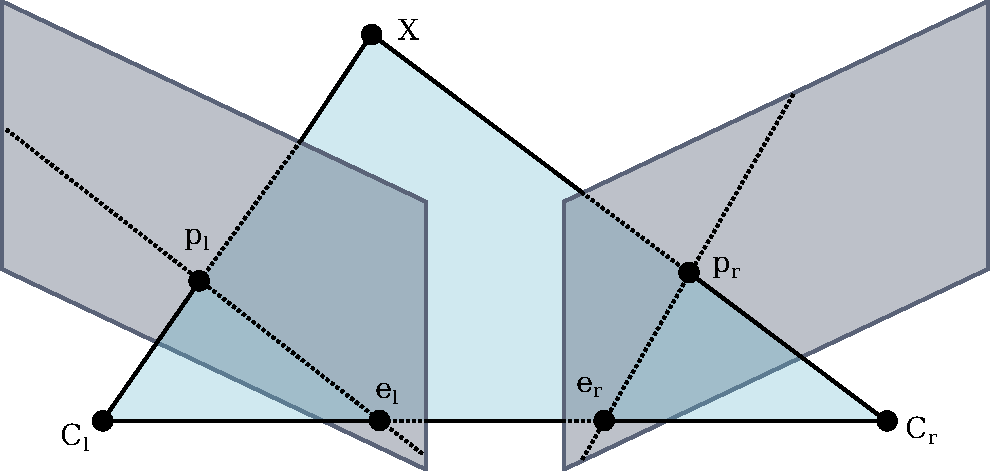
\includegraphics[width=\linewidth]{assets/img/epipolar.pdf}
	\caption{Epipolar constraint between two cameras.
	The center of the left and right cameras are $C_l$ and $C_r$,
	$X$ is the observed 3D point, projected onto $p_l$ and $p_r$
	respectively in the left and right image.
	The left and right epipoles are noted $e_l$ and $e_r$.}%
	\label{fig:epipolar}
\end{figure}

Alternatively to the stereo scheme, one can use a single camera.
It is called monocular visual odometry.
In that case, the 3D structure is unknown.
The relative motion between frames must then be retrieved
from the 2D information only.
That vector passing through the camera center and a given pixel of the image
is usually called a bearing vector.
In the monocular case, the motion and 3D structure computed by
visual odometry can only be recovered up to an unknown scale
when using the pinhole camera model.
This is due to the fact that the projection modelization cannot
differentiate big distances far away from small distances close to the camera.
The first influencial work exploiting monocular camera in a realtime algorithm
is the one of Nister et.\ al.~\cite{nister2004visual},
also coining the term ``visual odometry''.
It provides two important improvements over previous work.
First is the use of reprojection error,
which is the distance between the detected point in an image
and its reprojection from the 3D point with a given camera transformation,
while previous work tend to compute motion by aligning 3D point clouds.
The second is the use of a five-point minimal solver~\cite{nister2003efficient}
in a RANSAC scheme for robust motion estimation.

Recently, depth-sensing cameras such as the Microsoft Kinect~\cite{zhang2012microsoft}
have appeared in the consumer market under the name RGB-D cameras (``D'' for depth).
Those cameras use an active system based on structured infrared light
to compute a depth image.
Due to limitations in outside environments,
the usage of these cameras is restricted
to indoor navigation.
One should also avoid very reflective surfaces such as glass and mirrors.
In favorable cases, RGB-D cameras offer the advantage of providing
realtime depth information without the need of triangulation like in the stereo case.

One should note that in some situations, the camera can be paired
with other sensing devices.
Inertial measurement units (IMU) are present in smartphone
and LIDAR are often provided in autonomous vehicles for example.
Any additional information or constraint provided by a particular setup
can be exploited to improve performances of the visual odometry system.
There are therefore many papers exploring these areas but we will not discuss them here.

\subsection{Relation to Visual SLAM}%
\label{sub:relation-visual-slam}

Visual simultaneous localization and mapping is the name given to the technique
consisting in recovering the 3D structure of the environment (the map)
and the trajectory of the camera relative to this environment.
While visual odometry is only concerned with the local consistency of the
map and trajectory, visual SLAM tries to obtain a globally consistent map.
This difference is of the utmost importance for autonomous systems navigating
for a long period, but less so for short augmented reality experiences for example.

There exists three dominant strategies in visual SLAM.
One is based on filtering methods
such as in MonoSLAM by Davison et.\ al.~\cite{davison2007monoslam}.
Those approaches use methods similar to the extended Kalman filter (EKF)
to jointly estimate the camera trajectory and the 3D location
of a small number of landmarks in a probabilistic scheme.
The second strategy consists in keeping a small subset of the frames
called keyframes and apply global optimization algorithms such as
bundle adjustment on those.
One such example is the algorithm of Klein and Murray called
parallel tracking and mapping (PTAM)~\cite{klein2007parallel}.
Finally there are bio-inspired strategies such as RatSLAM
by Milfort et.\ al.~\cite{milford2004ratslam}.

Today, the majority of commonly used visual SLAM methods are keyframe-based.
The two most comprehensive solutions are ORB-SLAM~\cite{mur2015orb}
and OpenVSLAM~\cite{sumikura2019openvslam}.
Keyframe-based visual SLAM is usually composed of a visual odometry core,
extended with three components providing the global consistency.
A pose graph is built with the selected keyframes.
Camera locations are the nodes of the graph and transformations
between keyframes are stored in the edges.
A loop closure mechanism is added to detect when the camera
returns in previously visited locations.
When a loop is detected, an edge is added to the pose graph.
Finally, a global optimization such as bundle adjustment
is used to refine both keyframes camera locations
and estimated 3D points.
The choice between visual odometry and visual SLAM
is thus mainly a tradeoff between realtime performances
and accuracy and consistency over a long period of time.
In our work presented later in this document, we focus on visual odometry since
visual SLAM could be tackled later as an extension.

\subsection{Reducing Drift}%
\label{sub:reducing-drift}

\subsubsection{Outlier Removal with RANSAC}%
\label{ssub:ransac}

Random sample consensus (RANSAC) is a method to estimate
a model from a set of noisy data~\cite{fischler1981random}.
It consists in sampling a random subset of the data,
estimate a model from it,
and classify the rest of the data as fitting (inliers) or not (outliers) that model.
If we note $s$ the number of data points in the samples,
$\epsilon$ the percentage of outliers in all the data,
and $p$ the target probability of successfully find the correct model,
the number $N$ of samples required is
\[
	N = \frac{\log(1-p)}{\log(1 - (1 - \epsilon)^s)}.
\]
In a situation where 50\% of the data is outliers,
and with a target probability of success of 99\%,
it requires 16 iterations for a sampling size of 2 data points
and 145 iterations for a sampling size of 5,
growing at an exponential rate.
This is one reason why exploiting every available constraint of the system
to reduce the degrees of freedom is important.
As a consequence, a number of minimal model parameterizations
have been studied such as a three-point solver proposed by Fraundorfer et.\ al.\
when two of the camera angles are known~\cite{fraundorfer2010minimal}.
Using a robust estimation scheme like the one provided by RANSAC
can considerably reduce the drifts accumulated along the sequence.


\subsubsection{Windowed Bundle Adjustment}%
\label{ssub:windowed-ba}

Another method, complementary to outliers removal,
is to use windowed bundle adjustment.
The main issue of bundle adjustment, used in structure and motion
algorithms as well as in global optimization for visual SLAM,
is the computational complexity, growing in cube of the number of points
and camera poses.
Therefore, limiting bundle adjustment to a small ``window'' of frames
offers an efficient way of optimizing camera localization and 3D structure
with a controlled complexity.


\section{Motion Estimation}%
\label{sec:motion-estimation}

We have explained in Section~\ref{sub:3d_space_rigid_body_motion}
that the camera motion between two frames can be represented by
a transformation with 6 degrees of freedom (DoF) called rigid body motion
\[
	g(\bm{x}) = R\bm{x} + \bm{t},\quad R \in SO(3),\quad \bm{t} \in \R^3.
\]
In homogeneous coordinates, we can write
$g = \inmatrix{R & \bm{t}\\ 0 & 1}$.
The core challenge of visual odometry is to accurately estimate
this transformation $g$ from the observations provided by the camera images.
The two main approaches are feature-based or appearance-based.
Feature-based motion estimation is also sometimes called indirect,
while appearance-based is called direct visual odometry.
The distinction is due to the fact that feature-based methods
first step is to find and match features in the images.
Once features are paired, only their geometric information (location) is kept
to estimate the camera motion.
In contrast, direct (appearance-based) methods formulate the camera motion
estimation as a problem directly depending on the image intensity observations.


\subsection{Feature-Based Motion Estimation}%
\label{sub:feature-based}

There are three main feature-based approaches,
depending on the formulation of the feature correspondences.
A detailed presentation of each scheme is provided in the first part
of the visual odometry tutorial by Scaramuzza and Fraundorfer~\cite{scaramuzza2011visual}.

\subsubsection{3D to 3D}%
\label{ssub:3d_to_3d}
When features in previous and current frames have a depth information,
one can compare the points 3D coordinates.
There are two main strategies to estimate the motion from those point clouds.
The first is to consider point clouds globally and try to align them as a whole.
Variants of the ICP ``iterative closest point'' algorithm~\cite{besl1992method},
which is a method for registration of 3D shapes, are well suited for this task.
This strategy is often used in the case of RGB-D cameras since it avoids
the step of matching features in both images.

When features are matched, another strategy consists in
formulating the problem as a minimization problem
\[
	\arg \min_{g_k} \sum_{i} \| \bm{X}_k^i - g_k(\bm{X}_{k-1}^i) \|
\]
where $g_k$ is the rigid body motion between frames $k-1$ and $k$,
$\bm{X}_k^i$ and $\bm{X}_{k-1}^i$ are the 3D coordinates of point $\bm{X}^i$
in the camera frames $k$ and $k-1$.
This formulation is quite sensible to outliers so a robust approach is desirable.

\subsubsection{2D to 2D}%
\label{ssub:2d_to_2d}

When no depth information is provided by the sensors,
it may be preferable to avoid the estimation of 3D coordinates all together.
In presence of a calibrated camera, its motion can be recovered
thanks to the essential matrix
\[
	E = \cross{t}R
\]
where $t$ is the translation up to an unknown scale factor,
and $R$ is the rotation of the transformation.
The essential matrix itself is computed thanks to the epipolar constraint,
stating that for every matching pair of normalized image coordinates
$\bm{p}$ and $\bm{p}'$,
\[
	\tr{\bm{p}'}E\bm{p} = 0.
\]
The essential matrix can be recovered with factorization techniques~\cite{longuet1981computer}.
When robustness to outliers is desired,
the most common solution is to use a RANSAC-like scheme,
with a five-point algorithm such as the one presented by Nister~\cite{nister2003efficient}.

\subsubsection{3D to 2D}%
\label{ssub:3d_to_2d}

Instead of comparing 3D coordinates of triangulated points,
it is also possible to compare the reprojection of a 3D point $\bm{X}_{k-1}^i$
into the image $I_k$, that we will note $g_k(\bm{X}_{k-1}^i)$,
with its actual position in the image, noted $p_k^i$.
This error is usually called a reprojection error.
As we will explain soon, we can compute another kind of reprojection error,
based on appearance, so I will call this a geometric reprojection error.
Recovering the camera motion thus consists in minimizing the geometric reprojection error
\[
	\arg \min_{g_k} \sum_i \| p_k^i - g_k(\bm{X}_{k-1}^i) \|^2
\]
This problem is called ``perspective from n points'' (PnP).
The minimal case requires at least three points and is called
``perspective from three points'' (P3P).
A P3P solver may return up to four potential solutions
that can be disambiguated with other points.
In our interactive visual odometry Web application,
we provide a fast P3P implementation based on
Persson and Nordberg's solver~\cite{persson2018lambda}.

\subsection{Appearance-Based Motion Estimation}%
\label{sub:appearance-based}

Most appearance-based motion estimation methods are also direct,
with some exceptions like the algorithm by Goecke et al.~\cite{goecke2007visual}
which computes the Fourier-Mellin transform of the image.
Our implementation belongs to the direct image alignment category
so we will detail how this works.

\subsubsection{Direct Image Alignment}%
\label{ssub:direct-image-alignment}

In general, the direct approach formulates the problem as an
image registration (alignment) task.
Under the photoconsistency assumption, i.e.\ the appearance of a point
does not change between images, aligning them consists in
finding the transformation $W$ minimizing the photometric reprojection error
\[
	\argmin_{W} \sum_{\bm{x}}\|I(W(\bm{x})) - I^{*}(\bm{x})\|^2
\]
where $I^{*}, I$ are the reference and new images,
and $\bm{x}$ is the position of a pixel in the reference image.
The transformation $W$ is called the warp function and can take many forms.
Most of the time it is parametric, such as a 2D affine transformation,
visualized in Figure~\ref{fig:direct-image-alignment} and modelled
by the matrix $\inmatrix{
		1 + p_1 & p_3     & p_5 \\
		p_2     & 1 + p_4 & p_6}$
where $p_1$ to $p_6$ are the six parameters of the transformation.
The non parametric case is well known under the name optical flow
which consists in recovering the vector field describing the movement of all pixels.
To model the warp function by a rigid body motion of the camera capturing the image,
one could represent the camera motion by a matrix of the form $\inmatrix{R & \bm{t}}$
with $R \in SO(3)$ and $\bm{t} \in \R^3$.
The main inconvenience of this parameterization is that $R$ is a constrained 3x3 matrix,
so using 9 free parameters to optimize is clearly suboptimal.
Recent direct visual odometry algorithms seem to all agree on using
the Lie algebra $\seee$ for the parameterization of the rigid body
motion~\cite{newcombe2011dtam, audras2011real, kerl2013robust,
klose2013efficient, forster2014svo, engel2017direct}.

\begin{figure}[h]
	\centering
	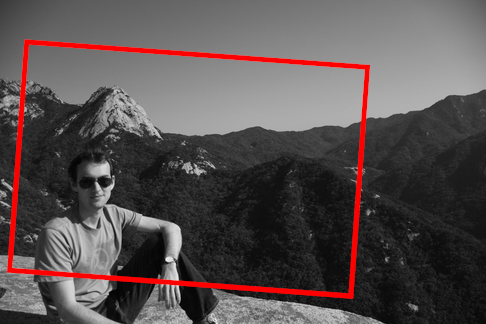
\includegraphics[width=0.48\linewidth]{assets/img/image-alignment-1.png}
	\hfill
	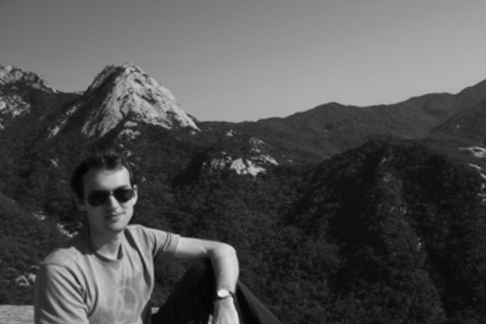
\includegraphics[width=0.48\linewidth]{assets/img/image-alignment-2.png}
	\caption{Direct image alignment. The 2D affine transformation between the first
	and second image is represented with the red rectangle.}%
	\label{fig:direct-image-alignment}
\end{figure}

\subsubsection{Minimization of the Photometric Reprojection Error}%
\label{ssub:minimization_photometric_error}

The minimization of the photometric reprojection error is a non-linear,
non-convex problem due to the form of the warping function.
It is common to solve it with a non-linear iterative algorithm such as Gauss-Newton.
If we add the parameterization to the notation, $W(\bm{x}) = W(\bm{x}, \bm{\xi})$,
and consider that $\bm{\xi}$ is to be found iteratively,
we can rewrite the expression to minimize as
\[
	\argmin_{W} \sum_{\bm{x}}\|I(W(\bm{x}, \bm{\xi} + \delta \bm{\xi})) - I^{*}(\bm{x})\|^2.
\]
In a Gauss-Newton scheme, the minimum is found by performing a first order
Tailor expansion of $I(W(\bm{x}, \bm{\xi} + \delta \bm{\xi}))$.
Using the chain rule, the gradient of this expression can be written
$J = \nabla I \nabla_{\bm{\xi}}W$ where $\nabla I$ is the image gradient
and $\nabla_{\bm{\xi}}W$ is the Jacobian of the warping function.
Let $H$ be the Gauss-Newton approximation of the Hessian,
$H = \sum_{\bm{x}}\tr{J}J$,
then the step of the parameters $\delta \bm{\xi}$ is given by
\[
	\delta \bm{\xi} = \inv{H} \sum_{\bm{x}} \tr{J} (I^{*}(\bm{x}) - I(W(\bm{x}, \bm{\xi})))
\]
and the new set of parameters is updated as $\bm{\xi} \leftarrow \bm{\xi} + \delta \bm{\xi}$.

In~\cite{baker2004lucas} Baker and Matthews provide a detailed review of the direct
alignment problem in a unifying framework showcasing the different possible formulations
of the expression to minimize.
Those formulations are referred to as forward additive, forward compositional,
inverse additive and inverse compositional.
The inverse additive approach is subtly different but the other three are
easily summarized by Table~\ref{tab:image-alignment-method}.
The compositional approaches model the increment as the composition
so it is required that the set of warps forms a group.
The inverse compositional approach exchange the roles of the reference image
with the new image to align.
This has a computational and accuracy advantage since the image gradients
are computed on the reference image $I^{*}$.
For this reason, the majority of direct visual odometry algorithms,
including our own implementation use that inverse compositional scheme.


\begin{table*}[ht]
\centering
\begin{tabular}{lll}
Formulation
	& Minimization
    & Warp update\\
    \midrule
Forward additive
	& $I(W(\bm{x}, \bm{\xi} + \delta \bm{\xi})) - I^{*}(\bm{x})$
	& $W(\bm{x}, \bm{\xi}) \leftarrow W(\bm{x}, \bm{\xi} + \delta \bm{\xi})$\\
Forward compositional
	& $I(W(W(\bm{x}, \delta \bm{\xi}), \bm{\xi})) - I^{*}(\bm{x})$
	& $W(\bm{x}, \bm{\xi}) \leftarrow W(\bm{x}, \bm{\xi}) \circ W(\bm{x}, \delta \bm{\xi})$\\
Inverse compositional
	& $I^{*}(W(\bm{x}, \delta \bm{\xi})) - I(W(\bm{x}, \bm{\xi}))$
	& $W(\bm{x}, \bm{\xi}) \leftarrow W(\bm{x}, \bm{\xi}) \circ \inv{W(\bm{x}, \delta \bm{\xi})}$\\
\end{tabular}

\caption{Formulation of the expression to minimize and the warp update step
	depending on the optimization scheme, as detailed in~\cite{baker2004lucas}.}%
\label{tab:image-alignment-method}
\end{table*}

\subsubsection{About the Depth Requirement}%
\label{ssub:depth_requirement}

Few words regarding the fact that the warping function needs the depth information
for the reprojection and why we thus tackled the easier RGB-D case.

\subsection{Extensions and Richer Modelizations}%
\label{sub:vo_extensions}

The purpose here is just mention a few existing things that we are not going to explain,
but should not be completely ignored such as:
robust, extensions to rolling shutter, continuous-time location, other cameras, photometric changes,
deep learning, event cameras, etc.
